% !TEX encoding = UTF-8 Unicode
%%%%%%%%%%%%%%%%%%%%%%%%%%%%%%%%%%%%%%%%%%%%%%%%%%%%%%%%%%%%%%%%%%%%%%%%%%%%%%%%%%%%%%%%%%%%%%%%%%%%%%% 
%%
%%  This file is asmeconf-template.tex, a LaTeX template to format ASME Conference papers according to
%%  the requirements on ASME's conference web pagess, and including hypertext support for the pdf.
%%
%%  This file is version 1.45 dated 2025/11/10
%%  
%%  As of version 1.11, this template defaults to ASME's newer conference guidelines first posted July 2019.
%% 			Those guidelines changed the author block formatting to be inline. 
%%			If you prefer the traditional grid format, use the class option [grid].
%%			Nomenclature now follows the abstract, and the abstract text is set in italics.
%%
%%  Author: John H. Lienhard, V
%%          Department of Mechanical Engineering
%%          Massachusetts Institute of Technology
%%          Cambridge, MA 02139-4307 USA
%%
%%  Class options include:
%%
%%          * An option to use the traditional grid arrangement of author names, [grid].  
%%			*	 With this option, line breaks (\\) may be inserted into the address as needed. 
%%			*	 Author names that include commas should be enclosed in braces, e.g.,  {Joseph L. Smith, Jr.}.  
%%			*	 Authors may be grouped above a single affiliation using braces, e.g., {Henry Tudor, Catherine Parr}.
%%
%%          * An option to balance the heights of columns on the last page, [balance]. 
%%
%%          * An option to include line numbers, [lineno]. You must *run twice* for proper placement of the line numbers. 
%%			*	 The lineno package does not number titles, footnotes, captions, or tables.
%%          *    This option will disable balancing column height on final page if that option has been invoked.
%%          *    The lineno package won't always number the lines preceding displayed math in a paragraph because
%%          *    paragraph has not ended.  See that package's documentation for macros to address this problem, or
%%          *    just leave a blank line above the displayed equation while you are editing and then remove the 
%%          *    blank line along with [lineno] option when you move to your final version.
%%
%%			* An option not to use a boldface font for caption text, [unboldcaption]
%%
%%          * Options to: 	omit the ASME copyright footer, [nofoot]; 
%%			*				use government employee copyright notice,      [govt];
%%			*				use government contractor copyright notice,    [contractor];
%%			*				use copyright notice for some gov't employees, [somegovt];
%%			*				omit the conference headers on the titlepage,  [nohead]
%%
%%			* Option to use LuaLaTeX **without** unicode-math and fontspec, [nofontspec]
%%
%%          * Math options from M. Sharpe's newtxmath package: upright integrals [upint]; 
%%          *    [varvw] for a v and w that are better distinguished from Greek nu; and also 
%%          *    [subscriptcorrection, smallerops, varg, frenchmath, varbb, cmbraces, slantedGreek,...] 
%%			* 	 See newtx documentation for descriptions (at CTAN: https://www.ctan.org/pkg/newtx, v1.744 or higher is best).
%%			*	 newtx is not loaded with lualatex unless the [nofontspec] option is used.
%%
%%          * An option to allow hyphenation of the typewriter font [hyphenate], from the inconsolata package (pdfTeX only).
%%          *    Hyphenation is normally suppressed for a typewriter (monospaced) font because those are often used for code.
%%			*	 To replace the default variable word spacing by monospacing, use the option [mono].
%%			*	 To get a zero without a slash, use [var0]
%%
%%			* PDF/A compliance:  Since 2022, LaTeX has included support for PDF/A, through the \DocumentMetadata{..} command.
%%
%%          * Options (used by the babel package) to include passages in languages other than English (e.g., a translation 
%%			*    of the abstract).  See Appendix C for details.
%%			*    	pdftex: Appropriate scripts will be loaded if you call the class options [greek], [russian], or [vietnamese].
%%			*    
%%			*    	lualatex: Language support is most extensive when running LuaLaTeX, which automatically loads fontspec.
%%			*		Non-Latin scripts require the [loadscripts] option, see Appendix C. 
%%			*	 	Be aware that you might need to install additional fonts for some languages.
%%			 
%%  The use of commands defined or modified by the asmeconf class is illustrated throughout this file. In particular, 
%%  ASME requires capitalized section headings, and as a result some care is needed when using macros in section headings,
%%  as also illustrated below.
%%
%%  Use an **up-to-date and complete** installation of LaTeX, such as TeX Live 2025 or later. 
%%		LaTeX formats earlier than 2022 are not fully supported.
%%
 %=========================================================
%% 
%% LICENSE: 
%%
%% Copyright (c) 2025 John H. Lienhard
%%
%% Offered under the MIT license: https://ctan.org/license/mit 
%%
%%%%%%%%%%%%%%%%%%%%%%%%%%%%%%%%%%%%%%%%%%%%%%%%%%%%%%%%%%%%%%%%%%%%%%%%%%%%%%%%%%%%%%%%%%%%%%%%%%%%%%% 

%%  RECOMMENDED pdf management code.
%%  This code was added to the LaTeX kernel in June 2022.
%% 		See https://www.latex-project.org/news/latex2e-news/ltnews35.pdf
%%  If you have problems with these lines, you can comment them out or, better, update your LaTeX format.

\DocumentMetadata{
	lang		= eng-US, 	% default
	pdfstandard	= A-3u,		% A-2b, A-2u, A-3b, A-3u. Check that your figures also meet the standard you choose.
	pdfversion	= 1.7, 		% an older version of PDF, but very widely supported
%	pdfversion  = 2.0, 		% default for LaTeX. Version 2.0 supports tagged PDF.
%	pdfstandard = { ua-2 , a-4f }, % run with lualatex and use a very recent LaTeX format (e.g., 2025/11/01)
%	tagging 	= on, 		% for producing tagged pdf
}

%%%%%%%%%%%%%%%%%%%%%%%%%%%%%%%%%%%%%%%%%%%%%%%%%%%%%%%%%%%%%%%%%%%%%%%%%%%%%%%%%%%%%%%%%%%%%%%%%%%%%%%

%% CLASS OPTIONS are described above. Change the options given below to meet your needs.
%% 
%%	 	NB: Remove the [colorlinks] option before *final* submission to ASME, to get black text for printing,
%%			but keep that option for electronic use.
%%
%%		NB: If you are not using the language options, * remove * them (together with Appendices C and D).
%%			Greek, cyrillic languages, and vietnamese if used, must be named as \documentclass options under pdftex.
%%			Spanish, german, and many others, if used, do not need to be named when the babel package is dated 2024 or later.
%%
%%		NB: the mathalfa option was dropped in v1.41; load the mathalpha package in your preamble instead.

\documentclass[colorlinks,upint,subscriptcorrection,varvw,hyphenate,balance]{asmeconf} % pdftex
\usepackage{tikz}
\usepackage{pgfplots}
\pgfplotsset{compat=1.18}
\usetikzlibrary{arrows.meta,positioning,calc,shapes.geometric}
\usepackage{dblfloatfix}
\usepackage{placeins}
\usepackage{float}
\usepackage{listings}

%\documentclass[colorlinks,upint,subscriptcorrection,varvw,balance,loadscripts,german,vietamese]{asmeconf} % lualatex

% Avoid aggressive vertical stretching between paragraphs/figures.
\raggedbottom
\setlength{\intextsep}{8pt plus 2pt minus 2pt}
\setlength{\textfloatsep}{8pt plus 2pt minus 2pt}
\setlength{\floatsep}{8pt plus 2pt minus 2pt}

%%%%%  pdf metadata  %%%%%%%%%%%%%%%%%%%%%%%%%%%%%%%%%%%%%%%%%%%%%%%%%%%%%%%%%%%%%%%%%%%%%%%%%%%%%%%%%%

\hypersetup{%
	pdfauthor={John H. Lienhard},									  % <=== change to YOUR name
	pdftitle={ASME Conference Paper LaTeX Template},                  % <=== change to YOUR pdf file title
	pdfkeywords={ASME conference paper, LaTeX template, BibTeX style},% <=== change to YOUR pdf keywords
	pdfsubject = {Describes the asmeconf LaTeX template},			  % <=== change to YOUR subject
%	pdfurl={https://ctan.org/pkg/asmeconf},% may delete
%	pdflicenseurl={https://ctan.org/pkg/asmeconf},% may delete
}
% If an author name or the title include a comma, enclosed it in braces, e.g., pdfauthor{John Forbes Nash{,} Jr.}


%%%%%%%%%%%%%%%%%%%%%%%%%%%%%%%%%%%%%%%%%%%%%%%%%%%%%%%%%%%%%%%%%%%%%%%%%%%%%%%%%%%%%%%%%%%%%%%%%%%%%%%

\allowdisplaybreaks % from amsmath package, allows multiline equations to break across pages (delete if not wanted)
					% using \\* instead of \\ will prevent specific lines from being pagebreaks.

% logos used in this document
\newcommand*\pdfTeX{pdf\TeX}    
\newcommand*\LuaLaTeX{Lua\LaTeX}
\newcommand*\BibTeX{Bib\TeX}

\begin{document}

% Change these fields to the right content for your conference.
% You can comment these out if for some reason you don't want a header.
% Use title case for the conference name (first letters capitalized), not all capitals

\ConfName{Proceedings of the ASME 2026\linebreak International Design Engineering Technical Conferences \&\linebreak Computers and Information in Engineering Conference}
\ConfAcronym{IDETC-CIE 2026}
\ConfDate{August 23--26, 2026}
\ConfCity{Houston, TX, USA}
\PaperNo{DETC2026-XXXX}

% Units of measure (e.g., cm) and other specialty lowercase terms in the title should be 
%   enclosed in \NoCaseChange{...} to maintain lower case type.
%   The rest of the title will automatically be set in all capital letters.
%
%	\title{Place Title Here: Place Subtitle After Colon} 

\title{Natural-Language to SysMLv2 Translation via Validator-Driven Iterative Refinement} % <=== replace with YOUR title
 
%   Put author names into the order you want. Use the same order for affiliations.
%   \affil{#} tags the author's affiliation to the address in \SetAffiliation{#}.
%   No space between last name and \affil{#}, separate names with commas.
%
%	For a sole author or a single affiliation for all authors, {#} may be left empty, i.e. \affil{} and \SetAffiliation{} (but not with [grid] option!)
%
%   \CorrespondingAuthor{email} follows that author's affiliation, no spaces before or after 
%   If multiple corresponding authors, put both email addresses in the same command and place after both authors.
%
%   \JointFirstAuthor, if applicable, follows the affiliation of the relevant authors, no spaces.

\SetAuthors{%
    Chance LaVoie\affil{1},
    Eladio Andujar Lugo\affil{1},
    Taylan G. Topcu\affil{2},
    Levent Burak Kara\affil{1}\CorrespondingAuthor{lkara@andrew.cmu.edu}
}

\SetAffiliation{1}{Department of Mechanical Engineering, Carnegie Mellon University, Pittsburgh, PA 15213 USA}
\SetAffiliation{2}{Grado Department of Industrial and Systems Engineering, Virginia Tech, Blacksburg, VA 24061 USA}
%   Note: You can force a line break in the address using \\ 

%	To switch from inline author names to gridded names, use the [grid] option.

\maketitle

%%% Use this footnote for tracking various versions of your draft. Change text to suit your own needs. 
%%% \date{..} calls the same command. 

%%% Change the following to your keywords.  Keywords are automatically printed at the end of the abstract.
%%% This command MUST COME BEFORE the end of the abstract.
%%% If you don't want keywords, leave the argument of \keywords{} empty (or use the abstract* environment)

\keywords{Systems Engineering, Design Automation, AI/KBS, Software Agents/Systems, Design Representation}

%%%%%  End of fields to be completed. Now write your paper. %%%%%%%%%%%%%%%%%%%%%%%%%%%%%%%%%%%%%%%%%%%


%%%%%  ABSTRACT  %%%%%%%%%%%%%%%%%%%%%%%%%%%%%%%%%%%%%%%%%%%%%%%%%%%
%%
%% Abstract should be 200 words or less
\begin{abstract}

Model-Based Systems Engineering (MBSE) relies on formal SysMLv2 models as primary technical artifacts for representing requirements, structure, and behavior across the system lifecycle. With the standardization of SysMLv2 as a textual language, there is growing interest in translating natural-language engineering descriptions directly into executable models. However, for practical deployment, generated models must be accepted by industrial modeling environments, not merely satisfy context-free grammar constraints.
This paper presents a validator-driven framework for reliable natural-language–to–SysMLv2 translation that enforces production-level acceptance as a termination condition. The proposed system embeds a production SysMLv2 validator within a generate–validate–repair loop. Each candidate model is evaluated using a production compiler, and deterministic diagnostics are incorporated into subsequent revisions until zero validation errors are achieved. By using the production validator as the correctness oracle, the framework targets operational deployability rather than grammar plausibility alone.
We evaluate the approach on the full SysMBench prompt set comprising 151 prompts across four large language model backends, yielding 604 prompt–model cases. Single-shot generation achieves 51.16\% production-validation acceptance, whereas validator-guided refinement achieves 100.00\% acceptance across all cases. Convergence is rapid, with most recoverable failures resolved within a small number of repair cycles.
By elevating production validation from a post-processing check to a control mechanism within generation, this work converts probabilistic text outputs into validator-accepted SysMLv2 artifacts suitable for loading, visualization, and downstream engineering use. To support reproducibility and further research, we release a trajectory-level corpus of all refinement traces.


% Large language models (LLMs) cannot reliably generate production-ready SysMLv2 models from natural language. Although prior systems improve grammar-level validity using parser-based constraints, grammar conformance alone does not guarantee acceptance in industrial modeling environments, where model-wide constraints are enforced by production validators. This unreliability prevents direct deployment of NL-to-SysMLv2 generation in real MBSE workflows.

% We address this barrier by elevating production validation itself to the correctness oracle. We instantiate a validator-driven generate--validate--repair loop in which each candidate model is evaluated by a production SysMLv2 validator and iteratively refined from deterministic diagnostics until zero-error acceptance. Rather than optimizing grammar plausibility, the system enforces operational deployability as a termination invariant.

% We evaluate this framework on the full SysMBench prompt set (151 prompts) across four model backends (604 prompt--model cases). Single-shot generation achieves 51.16\% production-validation acceptance, whereas validator-guided refinement achieves 100.00\% acceptance across all cases. Convergence is rapid, with most recoverable failures resolved within a small number of repair cycles.

% By using the production modeling tool as the oracle, this work converts plausible LLM output into validator-accepted SysML artifacts suitable for loading, visualization, and downstream engineering use. We release a trajectory-level corpus of all refinement traces to support further research on reliability, repair dynamics, and deployment-scale NL-to-MBSE systems.
\end{abstract}

%%%%%%%%%  BODY OF PAPER %%%%%%%%%%%%%%%%%%%%%%%%%%%%%%%%%

\section{Introduction}


Model-Based Systems Engineering (MBSE) replaces document-centric workflows with model-centric engineering, where formal artifacts represent requirements, structure, behavior, and verification intent across the system lifecycle~\cite{estefan2008mbse,madni2018mbse}. By elevating the model to the primary technical authority, MBSE reduces cross-document reconciliation effort and improves traceability under change~\cite{madni2018mbse,incoseSEVision2035}. SysMLv2 strengthens this transition by standardizing a formal language with complementary textual and graphical representations and machine-readable artifacts under the Object Management Group~\cite{omgSysMLv2Spec2024}. In practice, engineers can author the same model textually, render it visually, and exchange it across tools with reduced ambiguity. Because SysMLv2 is formal and textual, model construction is inherently scriptable. This scriptability creates an opportunity to translate natural-language engineering descriptions directly into executable SysMLv2 artifacts. However, for such translation to be useful in practice, generated models must be accepted by industrial modeling environments, not merely resemble well-formed text.

Recent advances in large language models (LLMs) suggest that automated generation can meaningfully accelerate engineering workflows. In software engineering, controlled and field studies report substantial productivity gains from LLM-assisted generation, including 55.8\% faster task completion, 26.08\% higher weekly completed tasks in enterprise randomized deployments, and measurable increases in pull-request throughput~\cite{peng2023copilot,cui2025highSkilled,demirer2024fieldCopilot}. These results motivate analogous integration in MBSE, where automating low-value authoring steps could increase modeling speed and allow teams to focus on architectural and verification reasoning. 

\textbf{Current State in MBSE:} Despite this opportunity, LLMs do not reliably produce production-validator-accepted\footnote{Production-validator-accepted: accepted by the production SysMLv2 validator with zero reported errors, indicating tool-level operational usability rather than grammar validity alone.} SysMLv2 models in single-shot generation. In response to this shortcoming, recent work has proposed structured pipelines for natural-language--to--SysMLv2 generation~\cite{bouamra2025systemp,cibrian2025sysmlagent}. SysTemp employs a template-first multi-agent design in which a template generator constructs a structured skeleton and a parser agent iteratively corrects syntax using grammar feedback~\cite{bouamra2025systemp}. Cibrián et al.\ organize generation as an agentic loop with a retrieval-augmented context engine and ANTLR-based grammar validation as the primary syntax gate~\cite{cibrian2025sysmlagent}. In parallel, SysMBench establishes a benchmark for evaluating natural-language--to--SysML generation quality, especially with respect to semantic alignment~\cite{jin2025sysmbench}. Collectively, these efforts demonstrate that grammar-conforming SysMLv2 can be produced from natural language.

\textbf{Limits of Grammar-Level Validation:} Despite this progress, grammar-level validity does not guarantee operational usability. Context-free grammar parsing ensures correct token ordering, balanced delimiters, and production-rule-compliant declarations. Industrial validators enforce additional model-wide constraints, including name resolution, type consistency, ownership rules, multiplicity constraints, and cross-reference integrity. A model that passes ANTLR parsing can still fail production validation and therefore remain unusable for visualization, simulation, or downstream analysis. In an auxiliary repository demonstration, highlighted in Appendix A, we show ten distinct examples that pass SysML ANTLR parsing yet fail production validation~\cite{sysmbenchCompilerLoopRepo2026}. The gap is therefore not grammar feasibility, but reliable generation of production-validator--accepted SysMLv2 from arbitrary natural-language prompts.

\textbf{Proposed advance:}
In this work, we present a validator-driven framework for natural-language--to--SysMLv2 generation that requires every generated model to pass a production validator before it is considered complete. We place a production SysMLv2 validator, SysIDE~\cite{sensmetry2024syside}, inside a generate--validate--refine loop. Given a natural-language prompt, the system produces a full textual SysMLv2 model and immediately checks it using the production validator. The reported diagnostics, such as unresolved references, typing errors, and ownership violations, are then used to revise the model. We repeat this process until the validator reports zero errors.

This approach follows the general idea of oracle-guided refinement from formal methods and inductive synthesis~\cite{clarke2000cegar,solarlezama2008thesis,jha2010ogis,alur2013sygus}, and is similar in spirit to compiler-feedback-driven code generation~\cite{wang2022compilable,grubisic2024compiler}. The difference here is that the oracle is a production modeling tool rather than a grammar parser. As a result, the loop enforces the same model-wide checks that an engineer would encounter when loading the model into an industrial environment.

We evaluate the framework on the full SysMBench prompt set of 151 prompts across four model backends, yielding 604 prompt--model cases. In single-shot generation, 51.16\% of the initial models pass production validation. With validator-guided refinement, all 604 cases reach zero-error acceptance, with most resolving in only a few repair cycles. These results show that production-validator feedback provides a reliable signal for correcting generated SysMLv2 models and makes direct integration into MBSE workflows feasible.

% \textbf{Proposed advance:} In this work, we present a validator-driven framework for natural-language--to--SysMLv2 generation that enforces production acceptance as the convergence criterion. We embed a production SysMLv2 validator, SysIDE~\cite{sensmetry2024syside}, inside a generate--validate--refine loop. At each iteration, the system generates a complete SysMLv2 candidate, evaluates it using the production validator, and conditions the next revision on deterministic diagnostics until zero validation errors are achieved. This design follows established oracle-guided refinement paradigms from formal methods and inductive synthesis~\cite{clarke2000cegar,solarlezama2008thesis,jha2010ogis,alur2013sygus} and aligns with compiler-feedback-driven code generation~\cite{wang2022compilable,grubisic2024compiler}. By elevating production validation from a post-processing check to a control operator within generation, our framework transforms plausible SysML text into deployable modeling artifacts suitable for loading, rendering, and downstream verification workflows.

Our main contributions are:
\begin{enumerate}
    \item A validator-in-the-loop architecture for natural-language--to--SysMLv2 translation that enforces production-validator acceptance as a termination invariant.
    \item A benchmark-scale empirical study across the full SysMBench prompt set and four model backends that quantifies the gap between grammar validity and production acceptance.
    \item A trajectory-level corpus of validator-guided refinement traces that enables future research on reliability, repair dynamics, and deployment-scale NL-to-MBSE systems.
\end{enumerate}

% Model-Based Systems Engineering (MBSE) replaces document-centric workflows with model-centric engineering, where formal artifacts carry requirements, structure, behavior, and verification intent across the lifecycle~\cite{estefan2007mbseSurvey,madni2018mbse,incoseMbseInitiative2025,sebokMBSE2025}. By making the model the primary technical source, MBSE reduces cross-document reconciliation overhead and improves traceability under change~\cite{madni2018mbse,incoseSEVision2035}.

% SysMLv2 strengthens this transition by standardizing a formal language with complementary textual and graphical representations and machine-readable artifacts under OMG~\cite{omgSysMLv2Spec2024,omgSysMLv2About2025,omgSysMLv2FinalAdoption2025}. In practice, the same model can be authored as text, rendered visually, and exchanged across tools with less ambiguity. Because SysMLv2 is formal and textual, model construction is scriptable.

% This scriptability, combined with the recent rise of LLMs in engineering practice, creates a concrete opportunity for automated SysMLv2 modeling workflows. LLM-based pipelines can generate candidate models directly from natural-language inputs.

% Software engineering provides encouraging precedent: controlled and field studies report substantial productivity gains from LLM-assisted generation, including 55.8\% faster task completion, 26.08\% higher weekly completed tasks in enterprise randomized deployments, and measurable increases in pull-request throughput~\cite{peng2023copilot,cui2025highSkilled,demirer2024fieldCopilot}. These results suggest that integrating generation into everyday tool use can materially accelerate engineering iteration.

% The analogous opportunity in MBSE is to automate low-value model authoring steps while increasing modeling velocity. If natural-language prompts can be converted into \emph{production-validator--accepted} SysMLv2, teams can spend less effort on syntax correction and more effort on architecture and verification reasoning.

% Despite this opportunity, large language models do not reliably generate production-validator--accepted SysMLv2 in single-shot settings. SysMLv2 is newly standardized, sparsely represented in public training corpora, and subject to strict industrial validation rules that enforce model-wide constraints beyond surface syntax. As a result, single-shot NL-to-SysMLv2 generation frequently produces artifacts that appear structurally plausible yet fail production validation.

% In response to this unreliability, recent SysMLv2 generation systems have moved beyond one-shot prompting toward structured generation workflows~\cite{bouamra2025systemp,cibrian2025sysmlagent}. SysTemp uses a template-first multi-agent design centered on a \textit{TemplateGeneratorAgent} and a \textit{ParserAgent}. A Jinja2-based template tool first builds a structured SysMLv2 skeleton, then a writer agent fills in content while parser feedback guides iterative correction~\cite{bouamra2025systemp}. By contrast, the 2025 \emph{Computers in Industry} framework organizes generation as an agentic loop with a RAG-based context engine and a validation engine, with ANTLR-based grammar validation as the syntax gate~\cite{cibrian2025sysmlagent}. In that framework, the context engine retrieves semantically similar natural-language prompt and SysML file pairs and exposes them to the LLM as context~\cite{cibrian2025sysmlagent}. Both approaches rely on context-free grammar (CFG) parsing as the primary basis for syntactic validation and as the primary acceptance metric.

% In parallel, SysMBench has established a common benchmark for evaluating natural-language--to--SysML generation quality, especially on semantic alignment criteria~\cite{jin2025sysmbench}. Read together, the current state of the art suggests that generating SysMLv2 from natural language that passes grammar-parser checks is feasible.

% Grammar parsability guarantees structural conformance to SysMLv2 context-free syntax: valid token ordering, balanced delimiters, and production-rule-compliant declarations. It does \emph{not} guarantee production validation acceptance, because industrial validators enforce additional model-wide constraints such as name resolution, type consistency, ownership/composition rules, multiplicity constraints, and cross-reference integrity. Therefore, parser-passing outputs provide no assurance that they will be accepted by a production modeling environment for downstream use, including visualization, semantic validation, simulation, and optimization. Without acceptance under a full industrial validator, such models remain unusable in practice. In an auxiliary repository demonstration, we show ten distinct cases that pass SysML ANTLR parsing but fail production validation, empirically reinforcing this distinction~\cite{antlrVsSysideDemo2026}. The critical gap is reliable generation of \emph{production-validator--accepted} SysMLv2 from arbitrary natural-language prompts.

% To close this gap, we instantiate a generate--verify--refine workflow in which candidate SysMLv2 models are iteratively evaluated against a production validation backend and revised until acceptance. In domains where large corpora of production-validator--verified artifacts are limited or the language and validation ecosystem continue to evolve, validator-in-the-loop refinement provides a practical mechanism for improving correctness without requiring model weight updates. This paradigm is not novel in itself. It draws from established traditions in formal methods and inductive synthesis, where candidate artifacts are proposed, evaluated by an external oracle, and corrected using deterministic feedback from that oracle~\cite{clarke2000cegar,solarlezama2008thesis,jha2010ogis,alur2013sygus}. Our contribution is to operationalize this verification-driven pattern for natural-language--to--SysMLv2 generation under industry-facing acceptance criteria.

% Related work in code generation has already demonstrated the technical value of iterative verifier-in-the-loop refinement. Wang et al.\ show that deterministic compiler diagnostics can be used as structured correction signals in multi-stage neural code generation, improving acceptance of generated programs under executable checks~\cite{wang2022compilable}. Grubi{\v{s}}i{\'c} et al.\ similarly use compiler feedback to iteratively refine LLM outputs, treating validator responses as an explicit control signal for subsequent generations~\cite{grubisic2024compiler}. Taken together, these works establish the core mechanism we rely on: generate a candidate, evaluate it with a deterministic backend, feed diagnostics back into the next iteration, and repeat until the validator reports no remaining errors.

% We apply this principle directly to MBSE. Our framework places a production SysMLv2 syntax validator, SysIDE~\cite{sensmetry2024syside}, in the loop as a deterministic oracle, and generation proceeds until zero-error acceptance is achieved under that validator. At convergence, the resulting model is production-ready and operational within the modeling environment---loadable, renderable, analyzable, and suitable for downstream verification workflows. By elevating production-validator acceptance to the convergence criterion, SysMLv2 generation moves from syntactic plausibility to deployable modeling infrastructure, establishing a practical foundation for Copilot-like support in MBSE workflows.

\section{Related Work}

Our review focuses on three areas that intersect in this study: (1) natural-language--to--SysML model generation within MBSE, (2) grammar-constrained and structured synthesis methods for large language models, and (3) verifier- and tool-guided refinement loops for generated artifacts. These bodies of work collectively demonstrate the feasibility of structured model synthesis from natural language and the benefits of deterministic feedback, while also highlighting open questions regarding deployment-level acceptance in industrial modeling environments.

\subsection{Natural-Language to SysML Model Generation}

Recent research has explored the use of large language models to generate SysML and SysMLv2 artifacts directly from natural-language requirements. SysTemp~\cite{bouamra2025systemp} introduces a template-driven, multi-agent pipeline in which a structured model skeleton is first constructed and then refined through parser-guided correction. Cibri{\'a}n et al.~\cite{cibrian2025sysmlagent} propose an agent-based architecture that combines retrieval-augmented generation with ANTLR-based grammar validation to improve syntactic correctness. These systems demonstrate that structured prompting and iterative repair can substantially improve parser-level validity for SysMLv2 text.

Additional studies examine LLM behavior in SysML-related tasks more broadly. Wang et al.~\cite{wang2025sysmlbehaviorllmempirical} report empirical findings on the generation of SysML behavioral models and identify common inconsistencies and hallucinations in model structure. Other work investigates LLM-assisted interaction with SysMLv2 artifacts in engineering settings~\cite{dehart2024sysml_llm} and describes workflows in which generative AI is used to build and query MBSE models\textbf{CITATION?}~\cite{symam24138generativeaimbsemodels}. These contributions reflect a growing interest in integrating LLMs into model-centric engineering practice.

Earlier efforts relied on restricted natural-language subsets, rule-based extraction, or diagram-level heuristics to translate requirements into SysML models~\cite{li2021restrictednlsysmlmodels,kbs2022nlpsystemsengineeringsysml,mistry2024texttomodeltransformationsysml}. While effective in constrained settings, these approaches often required controlled vocabularies or domain-specific grammars. More recent work explores LLM-assisted semantic alignment and model integration across SysMLv2 artifacts~\cite{anonymous2025semanticalignmentsysmlv2,hendricks2025texttomodel_sysml}. Collectively, this literature establishes the technical feasibility of NL-to-SysML pipelines, but most evaluations emphasize grammar conformity or diagram-level correctness rather than production-tool acceptance. Our work complements these efforts by examining acceptance under a production validation backend as the primary reliability criterion.

\subsection{Grammar-Constrained and Structured Synthesis}

Grammar-constrained decoding and template-based generation have emerged as practical strategies for improving structural correctness in LLM outputs. Grammar-constrained decoding methods restrict token sequences to context-free grammars, thereby enforcing well-formed structural patterns without requiring model retraining~\cite{geng2023gcd,park2024grammaraligneddecoding,frontiers2024gcdie}. These approaches reduce malformed outputs and improve syntactic validity across a range of structured generation tasks.

Template-driven methods further guide generation by providing predefined structural scaffolds or repair templates\textbf{CITATION?}~\cite{huang2025_template_guided_program_repair}. In SysML contexts, template-first pipelines such as SysTemp~\cite{bouamra2025systemp} use structured model outlines to stabilize generation. Such methods are particularly useful for newly standardized or low-data languages.

While grammar and template constraints effectively address token-level validity, they do not necessarily enforce model-wide consistency or tool-specific constraints. Production modeling environments typically impose additional checks related to reference resolution, typing consistency, and cross-model integrity. As a result, grammar-level correctness represents an important but partial notion of validity. Our approach builds on structured synthesis methods while shifting the acceptance criterion from parser conformity to production-tool validation.

\subsection{Verifier- and Tool-Guided Refinement}

Iterative refinement using deterministic feedback has a long history in formal methods and program synthesis. Counterexample-guided abstraction refinement and oracle-guided synthesis frameworks use external checkers to iteratively improve candidate artifacts~\cite{clarke2000cegar,jha2010ogis,alur2013sygus}. In the context of large language models, Wang et al.~\cite{wang2022compilable} and Grubi{\v{s}}i{\'c} et al.~\cite{grubisic2024compiler} demonstrate that compiler diagnostics can serve as structured correction signals for generated code. Subsequent work extends this paradigm to test-driven and verifier-driven loops~\cite{ravi2025llmloop,sevenhuijsen2024vecogen,morvalho2025cegisprogramrepair,namin2024vermcts}.

Across these domains, a consistent pattern emerges: candidate artifacts are generated, evaluated by a deterministic backend, and revised until the backend reports success. In software engineering, the oracle is typically a compiler, test suite, or formal verifier. Our work instantiates this refinement pattern in the context of SysMLv2 MBSE, where the oracle is a production modeling tool. By aligning the termination condition with the same validation mechanism used in industrial environments, we extend verifier-guided refinement to model-based systems engineering and examine its effect at benchmark scale.

% \section{Related Work}

% Prior work relevant to our study spans SysMLv2 generation, grammar-constrained synthesis, and verifier-guided refinement. The common thread is iterative error correction, but methods differ in the validation oracle used to accept or reject generated artifacts.

% \subsection{LLM-Based SysML v2 Model Generation}
% Recent systems show that structured prompting and agent decomposition improve SysMLv2 generation from natural language. SysTemp~\cite{bouamra2025systemp} combines template construction and parser-guided repair in a multi-agent pipeline; syntactic acceptance is determined by CFG-level parsing. Cibri{\'a}n et al.~\cite{cibrian2025sysmlagent} use an agentic architecture with a RAG-based context engine and an ANTLR-based validation engine, again using grammar parsing as the primary syntax gate. These methods establish feasibility of parser-level acceptance and iterative repair, but their acceptance criterion remains grammar conformance rather than production-validator acceptance. As a result, parser-valid artifacts can still be rejected in production modeling environments.

% \subsection{Grammar-Constrained and Template-Based Structured Synthesis}
% Template-first generation and grammar-constrained decoding reduce token-level invalidity by forcing outputs toward well-formed CFG structure~\cite{bouamra2025systemp,cibrian2025sysmlagent}. This is effective for enforcing declarations, delimiters, and keyword ordering, and it is a meaningful baseline for low-data languages. However, CFG acceptance does not enforce model-wide checks such as reference resolution, typing consistency, ownership constraints, or cross-model integrity. For MBSE deployment, grammar validity is therefore necessary but insufficient: artifacts must also pass production validation before they are operational in modeling environments.

% \subsection{Validator-in-the-Loop and Verifier-Guided Generation}
% Verifier-guided refinement is established in code generation: Wang et al.~\cite{wang2022compilable} and Grubi{\v{s}}i{\'c} et al.~\cite{grubisic2024compiler} show that deterministic diagnostics can drive iterative correction of generated programs. These studies motivate our control structure but are centered on software-language ecosystems with mature corpora and different acceptance targets. In SysMLv2 MBSE, the deployment criterion is production-validation acceptance in modeling environments, not parser pass rate alone.

% Across these lines of work, our approach differs by elevating production-validator acceptance to a termination invariant and evaluating this criterion at benchmark scale (151 prompts across four backends).


\section{Methodology}


In this section, we describe the experimental design and the validator-in-the-loop procedure used to evaluate natural-language--to--SysMLv2 generation. We first define the paired study setup, and then detail the iterative generation and validation workflow.

\subsection{Study Objective and Paired Design}

Our goal is to evaluate whether placing a production validator inside the generation loop improves reliability relative to single-shot generation. Specifically, we ask: for the same natural-language prompt and the same language model, does iterative validator-guided refinement increase the rate of production validation acceptance? In this study, we focus strictly on syntactic and production-level validation.

The experimental unit is a single prompt--model pair. For each pair, we compare two conditions obtained from the same generation trajectory:
\begin{enumerate}
    \item \textbf{Baseline (single-shot):} the production-validation outcome of the initial model produced by the language model ($k=0$).
    \item \textbf{Pipeline (iterative):} the production-validation outcome after applying validator-guided repair until termination.
\end{enumerate}

Because both outcomes are derived from the same prompt and the same model instance, this paired design isolates the effect of iterative validator feedback. Prompt content and model identity remain fixed, and only the presence or absence of validator-driven refinement differs between conditions.

\subsection{Validator-in-the-Loop Generation Procedure}

We implement a generate--validate--repair workflow for natural-language--to--SysMLv2 translation. Given a prompt, the language model produces a complete textual SysMLv2 candidate. We then evaluate this candidate using a production validator. If validation errors are reported, we pass the deterministic diagnostics back to the model and request a revised candidate. This process continues until the validator reports zero errors.

Let $P$ denote the natural-language prompt, $M_t$ the SysMLv2 model generated at iteration $t$, and $V(\cdot)$ the production validator. The update at each iteration can be written as
\[
M_{t+1} = f\!\left(P, M_t, V(M_t)\right),
\]
where $f(\cdot)$ represents the model call conditioned on the prompt, the previous candidate, and the validator diagnostics. In practice, $V(M_t)$ returns structured error messages that identify unresolved references, typing inconsistencies, ownership violations, and other model-wide constraint failures. These diagnostics guide the subsequent revision.

\setcounter{figure}{1}
\begin{figure*}[!b]
\centering
\definecolor{promptCardBg}{RGB}{248,247,243}
\definecolor{promptAccentOne}{RGB}{69,97,140}
\definecolor{promptAccentTwo}{RGB}{44,138,100}
\definecolor{promptAccentThree}{RGB}{196,106,28}
\definecolor{promptMetaText}{RGB}{92,99,108}

\begin{tikzpicture}
\tikzset{
    promptcard/.style={
        draw=black!16,
        fill=promptCardBg,
        rounded corners=6pt,
        line width=0.45pt,
        align=left,
        inner xsep=7pt,
        inner ysep=7pt,
        anchor=north west
    }
}

\node[promptcard] (p1) at (0,0) {%
    \begin{minipage}[t][52mm][t]{0.274\textwidth}
    \raggedright
    {\footnotesize\bfseries\textcolor{promptAccentOne}{Compact Workflow Prompt}}\hfill
    {\footnotesize\color{promptMetaText}Prompt 85}\par
    \vspace{1pt}
    {\scriptsize\itshape\color{promptMetaText}Photography Technique}\par
    \vspace{3pt}
    {\fontsize{6.8}{8.2}\selectfont
    The system is designed to implement a camera information processing workflow. When a user selects a scene through the camera's viewfinder (viewPort), the system first focuses on the scene to obtain an image (Image). This image is then captured to generate a photograph (Picture). After the photograph is generated, the system displays it on the screen via the display port (displayPort).\par}
    \end{minipage}
};

\node[promptcard, right=3.4mm of p1] (p2) {%
    \begin{minipage}[t][52mm][t]{0.274\textwidth}
    \raggedright
    {\footnotesize\bfseries\textcolor{promptAccentTwo}{Spatiotemporal Simulation Prompt}}\hfill
    {\footnotesize\color{promptMetaText}Prompt 26}\par
    \vspace{1pt}
    {\scriptsize\itshape\color{promptMetaText}Vehicle Traffic}\par
    \vspace{3pt}
    {\fontsize{6.8}{8.2}\selectfont
    This system is designed for spatiotemporal simulation of the dynamic behavior of vehicles on roads at different moments. Users can define parameters such as the vehicle's mass, position, velocity, and acceleration, and, combined with the road's slope (angle) and surface friction coefficient, depict the state of the vehicle and the road at specific time points. The system supports snapshot recording at multiple moments within the simulation time series, enabling tracking of the vehicle's state transitions from start-up (on state), through the driving process, to shutdown (off state).\par}
    \end{minipage}
};

\node[promptcard, right=3.4mm of p2] (p3) {%
    \begin{minipage}[t][52mm][t]{0.274\textwidth}
    \raggedright
    {\footnotesize\bfseries\textcolor{promptAccentThree}{Safety-Critical Monitoring Prompt}}\hfill
    {\footnotesize\color{promptMetaText}Prompt 48}\par
    \vspace{1pt}
    {\scriptsize\itshape\color{promptMetaText}Medical Health}\par
    \vspace{3pt}
    {\fontsize{6.8}{8.2}\selectfont
    This system is designed to ensure high reliability and safety of the blood glucose meter during use. When the battery is depleted or cannot be charged, the system should be able to automatically detect the battery status and promptly alert the user to prevent failure to measure blood glucose levels due to battery issues, as well as potential treatment delays resulting from such failures. To prevent the aforementioned failure scenarios, the system requires the implementation of preventive measures for battery status, and it must have appropriate alarm and emergency response mechanisms in case of abnormalities in the blood glucose measurement function.\par}
    \end{minipage}
};

\draw[promptAccentOne, line width=1.7pt] ([xshift=5pt,yshift=-5pt]p1.north west) -- ([xshift=-5pt,yshift=-5pt]p1.north east);
\draw[promptAccentTwo, line width=1.7pt] ([xshift=5pt,yshift=-5pt]p2.north west) -- ([xshift=-5pt,yshift=-5pt]p2.north east);
\draw[promptAccentThree, line width=1.7pt] ([xshift=5pt,yshift=-5pt]p3.north west) -- ([xshift=-5pt,yshift=-5pt]p3.north east);
\end{tikzpicture}

\caption{Representative SysMBench prompt excerpts illustrating the variety and structure of the benchmark inputs. The examples show a compact workflow prompt (Prompt 85), a spatiotemporal vehicle-simulation prompt (Prompt 26), and a safety-critical monitoring prompt (Prompt 48).}
\label{fig:prompt_showcase}
\end{figure*}
\setcounter{figure}{0}



We use SysIDE (\texttt{syside check}) as the production validation oracle~\cite{sensmetry2024syside}. A run terminates only when the validator reports zero errors. This choice is motivated by the distinction between grammar-level parsing and production acceptance. In an auxiliary ten-case study included in our repository and appendix, we demonstrate that models can pass the HAMR SysML v2 ANTLR4 parser while still failing production validation, illustrating that grammar conformity alone does not ensure operational usability~\cite{sysmbenchCompilerLoopRepo2026,hamrSysmlParser2026,sysmlV2PilotImplementation2026}. By using the production validator as the acceptance criterion, we align the loop with the same checks encountered in an industrial modeling environment.

\begin{figure}[H]
\centering
\resizebox{\columnwidth}{!}{\input{gcr_loop}}
\caption{Validator-in-the-loop generate--validate--repair workflow. The prompt remains fixed for each case, and each revision is driven by deterministic validator diagnostics.}
\label{fig:gcr_loop_methods}
\end{figure}
\setcounter{figure}{2}


% \subsection{Study Objective and Paired Design}
% This study evaluates one question: for the same prompt and the same model, does validator-in-the-loop refinement increase production validation acceptance relative to single-shot generation? The scope is strictly syntactic.

% The experimental unit is one prompt--model pair. For each unit, we evaluate two paired conditions taken from the same run trajectory:
% \begin{enumerate}
%     \item \textbf{Baseline (single-shot):} production validation outcome for the initial candidate ($k=0$).
%     \item \textbf{Pipeline (iterative):} production validation outcome at the final available iteration after iterative repair.
% \end{enumerate}

% Because both outcomes are taken from the same prompt--model run, this design isolates the effect of iterative validator feedback while holding prompt content and model identity fixed.

% \subsection{Validator-in-the-Loop Generation Procedure}
% Our controller follows a generate--validate--repair workflow for natural-language--to--SysMLv2 generation. At each iteration, the model proposes a complete SysMLv2 candidate, the production validator returns deterministic diagnostics, and the next model call is conditioned on those diagnostics.

% Let $P$ denote the natural-language prompt, $M_t$ the generated candidate at iteration $t$, and $V(\cdot)$ the production validator. The update is
% \[
% M_{t+1} = f\!\left(P, M_t, V(M_t)\right),
% \]
% where $f(\cdot)$ is the model revision operator conditioned on validator feedback.

% \begin{figure}[H]
% \centering
% \resizebox{\columnwidth}{!}{\input{gcr_loop}}
% \caption{Validator-in-the-loop generate--validate--repair workflow. The prompt is fixed per case, and each revision is driven by deterministic validator diagnostics.}
% \label{fig:gcr_loop_methods}
% \end{figure}

% The production validator oracle is SysIDE validation (\texttt{syside check})~\cite{sensmetry2024syside}. A run is successful and terminates only when zero validation errors are reported.
% This oracle choice is additionally supported by an auxiliary ten-case demonstration in the repository showing pass under the HAMR SysML v2 ANTLR4 parser with production-validation failure, i.e., grammar conformity without operational acceptability~\cite{antlrVsSysideDemo2026,hamrSysmlParser2026,sysmlV2PilotImplementation2026}.

\subsection{Dataset and Outcome Extraction}
SysMBench provides paired natural-language prompts and ground-truth SysMLv2 models for benchmark evaluation~\cite{jin2025sysmbench}. In this study, we use the curated natural-language prompt set (IDs 1--151) as generation inputs because it was designed to stress SysMLv2 LLM generation across diverse modeling patterns.

To demonstrate the variety and structure of the SysMBench prompts, Figure~\ref{fig:prompt_showcase} shows three representative prompt excerpts demonstrating a compact photography workflow specification, a spatiotemporal vehicle traffic simulation prompt, and a safety-critical medical health monitoring prompt.

To assess model-agnostic behavior of the same controller, we run four model configurations: OpenAI Codex 5.2 (\texttt{gpt-5.2-codex})~\cite{openaiGPT52Codex2026}, Anthropic Sonnet 4.6 (\texttt{claude-sonnet-4-6})~\cite{anthropicSonnet46API2026}, DeepSeek Reasoner (\texttt{deepseek-reasoner})~\cite{deepseekReasonerAPI2026}, and Mistral Large (\texttt{mistral-large-latest})~\cite{mistralLargeLatestDocs2026}. This yields 604 prompt-level cases (151 prompts $\times$ 4 models).

From saved run records, we extract single-shot and pipeline pass/fail outcomes, iterations run, iterations to success, first/final error counts, cumulative error counts, per-iteration runtime, and token usage. For grammar-versus-production analysis, we also extract single-shot ANTLR parse pass/fail and single-shot SysIDE pass/fail from the same initial candidate artifacts for all 604 prompt--model cases. Error families are grouped from validator diagnostics (for example, parsing and reference errors), while warnings are tracked separately and do not change pass/fail labels.

\subsection{Evaluation Metrics}
\subsubsection{Production Validation Acceptance}
The primary evaluation metrics are production validation acceptance rates. For each analysis slice (overall and per-model), we report:
\begin{enumerate}
    \item single-shot pass rate (initial candidate, $k=0$),
    \item pipeline pass rate (final iteration of the validator-gated loop).
\end{enumerate}
\textbf{We also report iterations-to-success, defined as the number of repair cycles required for a prompt–model case to reach production-validator acceptance.}


\subsubsection{Grammar vs Production Validity}
To quantify the operational gap between grammar-level validity and production-validator acceptance, we compare ANTLR and SysIDE outcomes on the same single-shot artifact from each case. This comparison is performed on the initial candidate ($k=0$ in repair-cycle indexing).

Grammar validity is defined as ANTLR parse success using the HAMR SysML v2 ANTLR4 parser, which provides a generated grammar and Java parser/lexer derived from the SysML v2 Pilot Implementation~\cite{hamrSysmlParser2026,sysmlV2PilotImplementation2026}. This ANTLR check is used only as a representative context-free grammar (CFG) parsability test and does not enforce production model-wide constraints. Production validity is defined as SysIDE acceptance (zero SysIDE errors) under \texttt{syside check}. For each case, we record binary pass/fail outcomes for both checks and construct a $2\times2$ contingency table (ANTLR pass/fail $\times$ SysIDE pass/fail).

\subsubsection{Convergence Metrics}
To characterize how quickly the loop approaches acceptance, we index progress by repair cycles. Let $k=0$ denote the initial single-shot generation (no validator feedback), and let $k\geq 1$ denote $k$ rounds of generate--validate--repair. Let $A_k$ denote cumulative production-validation acceptance after repair cycle $k$.

We define residual failure mass as
\[
R_k = 1 - A_k,
\]
where $R_k$ is the fraction of prompt--model cases not yet accepted at repair cycle $k$. We then define an empirical contraction ratio
\[
\rho_k = \frac{R_{k+1}}{R_k}.
\]
When $0 < \rho_k < 1$, residual failure shrinks from one cycle to the next; when $\rho_k$ is approximately stable across $k$, the observed trajectory suggests contraction-like behavior, with approximately multiplicative reduction in the early repair regime under standard contraction-style analyses in iterative methods~\cite{banach1922operations,nocedal2006numerical,he2016averageConvergenceRate}.
In finite empirical campaigns, we estimate contraction behavior from early-to-mid cycles, before residual mass becomes very small; terminal transitions are excluded from rate estimation because finite-sample tail effects can produce unstable ratios near the finite-sample resolution.
This characterization is descriptive of observed finite-sample behavior and does not assert formal convergence guarantees.

We also report time-to-threshold acceptance
\[
T_{\varepsilon} = \min\{k : A_k \ge 1-\varepsilon\},
\]
with explicit reporting of $T_{90}$, $T_{95}$, and $T_{99}$. This follows standard iteration-to-threshold (iteration-to-$\varepsilon$) complexity summaries in optimization~\cite{polyak1987introductionOptimization}. These metrics provide an interpretable rate summary complementary to pass-rate metrics.

This framing follows empirical convergence-rate characterizations used in iterative optimization and search, including multiplicative (geometric-style) interpretations of residual reduction~\cite{he2016averageConvergenceRate}, while remaining descriptive rather than proving formal convergence guarantees. It is also consistent with iterative verifier-feedback refinement in code generation, where deterministic diagnostics guide successive corrections toward acceptance~\cite{wang2022compilable,grubisic2024compiler}.

\subsection{Statistical Reliability Analysis}
For convergence reliability, we model each prompt--model case as a Bernoulli success if it reaches eventual production-validator acceptance (zero SysIDE errors) within the allowed loop. Let $p$ denote convergence probability for prompts drawn from the SysMBench-style benchmark distribution under the same controller, validator, and backend configuration. Because the validator-gated loop is monotonic and accepted cases terminate immediately, regression transitions (single-shot pass $\rightarrow$ pipeline fail) are structurally excluded. Improvement is therefore quantified descriptively rather than via symmetric paired hypothesis tests.


We report an exact 95\% Clopper--Pearson lower confidence bound for $p$~\cite{clopper1934confidenceLimits}; in the all-success case this is $p_L=(\alpha/2)^{1/n}$ with $\alpha=0.05$. We also report the complementary one-sided 95\% binomial upper confidence bound on failure probability $q=1-p$. In the zero-failure case, this bound is obtained by solving $(1-q)^n=0.05$, yielding $q_U=1-0.05^{1/n}$. For large $n$, this expression is well approximated by $q_U\approx-\ln(0.05)/n\approx 3/n$.

These reliability bounds are intentionally scoped to SysMBench-style prompt distributions under the evaluated configuration and are reported numerically in Section~\ref{sec:results}. They are not treated as universal guarantees over arbitrary natural-language inputs.

\subsection{Extended Analyses}
\textbf{In addition to the primary evaluation metrics described above, we conduct several supplementary analyses to better understand repair behavior within the validator-guided generation loop. These analyses are presented in Appendix~B and Appendix~C. Specifically, we examine relationships between iterations-to-success and generated output length as well as SysMBench benchmark difficulty labels (Appendix~B). We also analyze persistent validator errors across repair iterations to characterize cases in which the language model fails to resolve a reported error despite attempting repair (Appendix~C). These analyses provide additional insight into repair dynamics and factors influencing convergence behavior.}

\subsection{Reproducibility}
All code, run artifacts, and analysis outputs used in this study are stored in the project repository~\cite{sysmbenchCompilerLoopRepo2026}. The repository includes the scripts required to regenerate campaign statistics, tables, and figures.


\section{Results}
\label{sec:results}

In this section, we present the results of our evaluation of production validation outcomes across the benchmark. We begin by examining overall acceptance behavior and then analyze reliability, convergence dynamics, and validation characteristics across models.


\subsection{Primary Outcome: Production Validation Acceptance}
Across all 604 prompt-level trials (151 prompts for each of four models), single-shot production validation succeeded for 309/604 cases (51.16\%). Under validator-in-the-loop refinement, pipeline production validation succeeded for 604/604 cases (100.00\%).

\begin{figure}[H]
\centering
% Figure 2 options (pick one):
% \input{results/figures/01_overall_option_b_dumbbell}
% \input{results/figures/01_overall_option_c_stacked_gain}
\input{results/figures/01_overall_option_a_horizontal}
\caption{Overall single-shot vs final pipeline production-validation acceptance across all 604 prompt-level cases.}
\label{fig:overall_baseline_vs_pipeline}
\end{figure}

\subsection{Per-Model Reliability}
All models reached 151/151 eventual production validation under the validator-gated loop, but single-shot pass rates differed substantially. Figure~\ref{fig:by_model_baseline_vs_pipeline} provides the per-model comparison with exact acceptance values annotated on the bars.

\begin{figure}[H]
\centering
\input{results/figures/02_baseline_vs_pipeline_compile_rate_by_model}
\caption{Per-model single-shot vs final pipeline production-validation acceptance.}
\label{fig:by_model_baseline_vs_pipeline}
\end{figure}

Anthropic Sonnet 4.6 had the highest single-shot pass rate (82.78\%), while OpenAI Codex 5.2 (41.72\%), DeepSeek Reasoner (41.06\%), and Mistral Large (39.07\%) showed worse single-shot behavior and larger single-shot-to-pipeline gaps.

\subsection{Convergence Behavior}
Convergence is indexed by repair cycles: $k=0$ denotes the initial single-shot generation (no validator feedback), and $k\geq 1$ denotes validator-guided repair cycles; acceptance corresponds to zero-error output under the production validator.

Figure~\ref{fig:cumulative_convergence} first presents the pooled convergence trajectory across all prompt-level cases.

\begin{figure}[H]
\centering
\input{results/figures/03_cumulative_acceptance_by_iteration}
\caption{Cumulative production-validation acceptance versus repair cycles ($k$). $k=0$ denotes initial single-shot generation; $k\geq 1$ denotes validator-guided repair cycles. Acceptance corresponds to zero-error output under the production validator.}
\label{fig:cumulative_convergence}
\end{figure}

The pooled curve shows a large first-step jump from $k=0$ to $k=1$, followed by rapid compression by $k=2$ and then a short tail. Table~\ref{tab:convergence_behavior} provides the exact counts and percentages underlying Figure~\ref{fig:cumulative_convergence}: acceptance increases from 51.16\% at $k=0$ to 84.44\% at $k=1$, reaches 94.37\% by $k=2$, and reaches 99.67\% by $k=4$. Only two cases remain in the grouped $k=5$--$8$ tail (0.33\%), where cumulative acceptance reaches 100.00\%. Consistent with this front-loaded pattern, iterations-to-acceptance are summarized by mean 1.727, median 1, IQR 1--2, and maximum 8.

\input{results/tables/table_convergence_behavior}

\noindent\textbf{Rate Characterization.} To quantify the observed convergence shape, we report an empirical contraction analysis of residual failure mass. Under contraction-style iteration analysis, let residual failure mass be $R_k = 1 - A_k$. The observed residual sequence is $R_0=0.4884$, $R_1=0.1556$, $R_2=0.0563$, $R_3=0.0182$, and $R_4=0.0033$. Using early cycles, the empirical contraction ratios are $\rho_0 \approx 0.1556/0.4884 \approx 0.32$, $\rho_1 \approx 0.0563/0.1556 \approx 0.36$, and $\rho_2 \approx 0.0182/0.0563 \approx 0.32$. These values cluster around an average early-cycle contraction factor of approximately 0.33 (computed as the arithmetic mean of $\rho_0$--$\rho_2$). Tail transitions are excluded from contraction-rate estimation because ratios become unstable when residual mass is near the finite-sample resolution. These early-cycle ratios cluster in a narrow band, suggesting an approximately multiplicative (``contraction-like'') reduction pattern in the initial repair regime. In practical terms, early cycles remove roughly two-thirds of the remaining failures per cycle (in the observed early regime).

Complementing the contraction estimate, time-to-threshold metrics quantify convergence speed. The observed thresholds are $T_{90}=2$, $T_{95}=3$, and $T_{99}=4$. These values characterize how rapidly validator-guided refinement approaches the acceptance set in repair-cycle space.

To assess whether this pooled behavior is shared across backends, Figure~\ref{fig:cumulative_convergence_by_model} overlays per-model cumulative acceptance trajectories.

\begin{figure}[H]
\centering
\input{results/figures/04_cumulative_acceptance_by_model_overlay}
\caption{Per-model cumulative production-validation acceptance versus repair cycles ($k$).}
\label{fig:cumulative_convergence_by_model}
\end{figure}

Figure~\ref{fig:cumulative_convergence_by_model} shows that single-shot starting points differ across models, but the trajectories compress rapidly once validator-guided repair begins. Despite different initial acceptance levels, all curves move quickly toward full acceptance within a small number of repair cycles. This pattern supports the model-agnostic control-signal interpretation: deterministic validator diagnostics drive the dominant convergence dynamics across backends.

\subsection{Statistical Reliability}

We now quantify the reliability of validator-guided convergence across the full campaign. In total, we evaluated $n=604$ prompt--model cases. In single-shot generation, 309 of 604 cases (51.16\%) passed production validation. Under validator-guided refinement, all 604 cases ultimately reached zero-error production acceptance, with no observed failures.

To interpret this result statistically, we model convergence as a Bernoulli process and compute an exact 95\% Clopper--Pearson lower confidence bound on the convergence probability $p$~\cite{clopper1934confidenceLimits}. For the all-success case ($x=604$ successes in $n=604$ trials), the lower bound is
\[
p_L = (\alpha/2)^{1/n},
\]
with $\alpha=0.05$. Substituting $n=604$ gives
\[
p_L = (0.025)^{1/604} \approx 0.9939.
\]
With 95\% confidence, the true convergence probability under this benchmark configuration is therefore at least 99.39\%.

Equivalently, we can compute a one-sided 95\% upper bound on the failure probability $q=1-p$ by solving $(1-q)^n=0.05$. For $n=604$, this yields
\[
q_U = 1 - 0.05^{1/604} \approx 0.00495,
\]
or approximately 0.495\%. A large-$n$ approximation gives $q_U \approx -\ln(0.05)/604 \approx 0.00496$, which is consistent with the exact calculation. 

In practical terms, this means that even though we observed zero failures in 604 cases, statistical uncertainty remains finite. Based on the binomial confidence analysis, we can state with 95\% confidence that the true failure rate under this benchmark configuration is below approximately 0.5\%, and equivalently that the true convergence probability exceeds 99\%. While this does not imply perfect reliability, it indicates that production-validator convergence is highly probable for SysMBench-style prompts under the evaluated setup.

We emphasize that these bounds apply to SysMBench-style prompt distributions under the evaluated controller, validator, and backend configuration. They do not imply universal convergence over arbitrary natural-language inputs. At the same time, the absence of observed failures is consistent with the structure of the loop. Accepted cases terminate immediately, and rejected cases receive deterministic diagnostics that guide subsequent revisions. Within this benchmark distribution, validator-gated refinement exhibits stable and highly reliable convergence behavior.

\subsection{Grammar Validity vs. Production Validity and Error Burden}

In practice, a SysMLv2 artifact must pass production validation in a modeling environment before it can be used downstream. Grammar parsability alone is not sufficient. To quantify the gap between these two notions of validity, we compared ANTLR parsing outcomes against production validation outcomes for the initial candidate ($k=0$) across all 604 prompt--model cases.

Of the 604 initial candidates, 369 (61.09\%) passed grammar-level parsing, whereas only 309 (51.16\%) passed production validation. In 60 cases, the generated model passed ANTLR parsing but failed production validation. These 60 cases represent 16.26\% of grammar-valid artifacts (60/369) and 9.93\% of all initial outputs (60/604). In other words, grammar-level parsing overestimates operational usability by approximately 16\% among parseable artifacts. We did not observe any case in which a model passed production validation while failing grammar parsing (0/604), indicating that grammar validity is necessary but not sufficient for production acceptance under the evaluated configuration.

\begin{figure}[H]
\centering
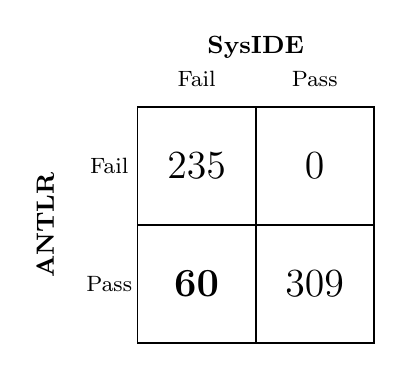
\begin{tikzpicture}[x=1.5cm,y=1.5cm]
\draw[line width=0.65pt] (0,0) rectangle (2,2);
\draw[line width=0.65pt] (1,0) -- (1,2);
\draw[line width=0.65pt] (0,1) -- (2,1);

% Axis labels and definitions
\node[font=\small\bfseries] at (1.0,2.50) {SysIDE};
\node[font=\footnotesize] at (0.5,2.24) {Fail};
\node[font=\footnotesize] at (1.5,2.24) {Pass};

\node[font=\small\bfseries, rotate=90] at (-0.78,1.0) {ANTLR};
\node[font=\footnotesize, align=right] at (-0.24,1.5) {Fail};
\node[font=\footnotesize, align=right] at (-0.24,0.5) {Pass};

% Cell values (top row: ANTLR fail, bottom row: ANTLR pass)
\node[font=\Large] at (0.5,1.5) {235};
\node[font=\Large] at (1.5,1.5) {0};
\node[font=\Large] at (0.5,0.5) {\textbf{60}};
\node[font=\Large] at (1.5,0.5) {309};

\end{tikzpicture}
\caption{Initial-candidate grammar (ANTLR) vs production validation (SysIDE), $n=604$. The operational-gap cell (ANTLR pass, SysIDE fail) contains 60 cases.}
\label{fig:antlr_vs_production_flow}
\end{figure}



%We also examined the validator error burden for initial candidates. Across all 604 cases, the production validator reported a total of 2,209 errors, corresponding to a mean of 3.66 errors per generated model. Restricting to the 295 cases that failed production validation, the mean error burden increases to 7.49 errors per failing model. These values indicate that failures typically involve multiple structural inconsistencies rather than isolated formatting mistakes.

%The distribution of error types further clarifies this pattern. Parsing errors account for 1,144 of the 2,209 total errors (51.79\%), while reference errors account for 824 (37.30\%). Together, these two categories comprise 89.09\% of all initial-candidate errors. This concentration suggests that many initial outputs contain compound structural defects, including unresolved references and incomplete declarations. Grammar-level parsing alone would admit a subset of these artifacts into downstream workflows, despite their inability to pass production validation. Validator-guided repair therefore addresses not only token-level syntax issues, but broader structural inconsistencies that affect operational usability.


\subsection{Insights from Extended Analyses}
\textbf{First, we observe no meaningful relationship between iterations-to-success and either SysMBench difficulty or the length of the generated SysML output. Repair effort therefore does not appear to scale with model size or benchmark difficulty. One possible explanation is that raw line count does not capture the number of distinct grammatical structures that must be correctly formed; shorter outputs may still contain complex reference or typing relationships that trigger validator failures.
Second, when validator errors persist across repair iterations, the majority occur because the LLM does not modify the validator-highlighted code region at all, effectively ignoring the reported diagnostic. In the remaining cases, the model appears to attempt a repair but produces another invalid construction. This pattern suggests both a pipeline efficiency gap, in which repair iterations are wasted when the highlighted region is not revised, and a model limitation, in which the model attempts a repair but fails to generate a syntactically valid correction.}

\subsection{Open-Source Dataset Release}

We release the full trajectory-level corpus generated in this study rather than only baseline and final artifacts. The dataset spans the complete SysMBench prompt set of 151 prompts evaluated across four model backends, yielding 604 prompt--model cases. For each case, we retain every validator-guided refinement step. In total, the release contains 1,043 stored iteration artifacts. Each artifact includes the generated SysMLv2 text and the corresponding production-validator diagnostics. As a result, the dataset preserves the full correction trajectory for each case, not just its endpoints.

At the artifact level, we classify iterations as positive if they pass production validation and negative if they fail. Under this definition, the release contains 604 positive artifacts and 439 negative artifacts. For a newly standardized language such as SysMLv2, where publicly available corpora of production-accepted models remain limited, these 604 positive artifacts provide a meaningful resource. The 439 negative artifacts correspond to intermediate repair states within the same 604 trajectories; they do not represent additional independent benchmark instances, but rather the correction path taken for each prompt--model pair.

%The negative artifacts are rarely trivial failures. Across all iteration artifacts, the validator reports 3,232 total error instances. When restricted to failing artifacts only, the mean error burden is 7.36 errors per artifact, with a median of 4.00 and a maximum of 267 errors in a single case. The maximum observed trajectory depth is eight iterations, and the mean number of iterations per case is 1.73. These statistics indicate that failing states typically involve multiple structural inconsistencies rather than isolated formatting issues, and that repair often requires resolving several interacting errors.

Releasing full stepwise traces enables analyses that are not possible with endpoint-only datasets. Researchers can study repair dynamics under deterministic validator feedback, model convergence behavior across trajectories, and explore learning strategies that operate on intermediate states rather than final outputs alone. Because we retain runtime and token-level metadata at both iteration and trajectory levels, the dataset also supports systematic cost--reliability tradeoff analyses under a consistent production-validation criterion.


\section{Discussion}

\textbf{Production Validation:} By placing a production validator inside the generation loop, we address a practical barrier to using natural-language--to--SysMLv2 generation in real MBSE workflows. Rather than producing text that appears structurally plausible, we require that every generated model satisfy the same production checks needed to load and use it in an industrial modeling environment. Across 604 prompt--model cases, validator-guided refinement increases production-validation acceptance from 51.16\% in single-shot generation to 100.00\%. In doing so, we remove the primary syntactic obstacle to integrating LLM-assisted modeling into existing toolchains.

\textbf{Reliability Mechanism:} Shifting from single-shot generation to validator-guided refinement also changes where reliability is enforced. In the single-shot setting, acceptance depends on whether the language model happens to produce a structurally correct artifact on its first attempt. In the validator-guided setting, we instead rely on a deterministic backend that evaluates and reports concrete modeling errors. At each iteration, we check the candidate model, revise it based on explicit diagnostics, and re-evaluate it until no validation errors remain. Because we apply the same production validator across all runs, acceptance becomes largely independent of backend-specific first-pass behavior. Model providers may differ in cost and latency, but we enforce production acceptance through a shared validation layer.

\textbf{Deployment Implications:} From a deployment perspective, we believe this distinction is critical. In typical MBSE environments, engineers must load, render, and validate models before using them for visualization, simulation, or verification. Without validator guidance, generated models are usable only when they happen to meet these constraints. With validator guidance, we enforce usability as part of the generation process itself. This allows us to incorporate LLM-assisted modeling into day-to-day engineering practice while maintaining bounded operational risk. In this setting, engineers can spend less time correcting structural syntax errors and more time reasoning about architecture, requirements, and verification intent.

\textbf{Convergence Dynamics:} The observed convergence behavior further supports this interpretation. Deterministic diagnostics provide stable correction signals, and we find that most recoverable failures resolve within a small number of repair cycles ($T_{90}=2$, $T_{95}=3$, $T_{99}=4$). Initial candidates often contain multiple structural errors, yet the loop typically resolves these issues in only a few iterations. These results suggest that the refinement process corrects shallow but compound structural inconsistencies rather than exhibiting unstable or oscillatory dynamics.

\textbf{Scope Limits:} We emphasize that the scope of these results is intentionally limited. By enforcing production validation, we guarantee structural and operational compatibility with a modeling tool, but we do not guarantee that the resulting model faithfully represents the intended system or satisfies its requirements. We do not evaluate semantic correctness, behavioral adequacy, or trace completeness in this study. In addition, we bound our empirical findings to the SysMBench prompt distribution and to a single production validator backend.

Within these bounds, we view validator-driven refinement as a foundational reliability layer for AI-assisted MBSE. Once we guarantee structural acceptance, we can introduce additional mechanisms such as semantic validation, cross-view consistency analysis, simulation-based checks, and requirement trace evaluation. By establishing production-validator acceptance as a stable baseline, we create a controlled starting point for building higher-level assurances on top of syntactic convergence.

% \section{Discussion}
% The central contribution is infrastructural: using the production validator as the generation oracle makes NL-to-SysMLv2 operationally deployable rather than merely plausible. Under this architecture, candidate text is transformed into production-acceptable model artifacts before handoff to engineering tools. Quantitatively, this shift moves acceptance from 51.16\% single-shot to 100.00\% final pipeline acceptance across the same 604 prompt--model cases, removing the primary syntactic barrier to direct MBSE workflow integration.

% This is a systems-level design move, not just iterative repair. Production validation is elevated from a post-processing check to a control operator inside generation itself. Reliability is therefore enforced at the workflow level through oracle-gated refinement, rather than left to backend-specific first-pass behavior alone. In practice, this decouples deployment reliability from model-provider choice: backend differences remain important for cost, latency, and governance, but acceptance control is implemented in the surrounding orchestration layer.

% The deployment consequence is concrete. Without oracle gating, NL-to-SysMLv2 output is probabilistically usable; with validator gating, it becomes conditionally deployable under explicit acceptance criteria. This allows MBSE environments to integrate LLM generation with bounded operational risk and supports Copilot-like modeling workflows in which analysts spend less time on structural syntax repair and more time on architecture, requirements reflection, and verification intent.

% Convergence behavior supports this interpretation without requiring stronger claims. Deterministic diagnostics provide stable correction signals, and most recoverable failures resolve in few cycles ($T_{90}=2$, $T_{95}=3$, $T_{99}=4$). Together with the observed first-failure error burden, this suggests the loop is typically resolving shallow but multi-error structural defects.

% Scope boundaries are clear. These results establish syntactic and operational reliability under production validation; they do not establish semantic correctness, architectural adequacy, or requirement satisfaction. Production-validation acceptance is necessary for deployability but not sufficient for engineering quality, and external validity remains bounded to one benchmark prompt distribution and one production validator backend.

% Within those bounds, validator-driven reliability can be treated as the first layer of an assurance stack for AI-enabled MBSE. This layer can support future agentic workflows that add higher-level guarantees for semantics, architecture, and traceability on top of enforced syntactic convergence.

\section{Conclusion}

Our results indicate that single-shot LLM generation does not reliably produce SysMLv2 models that pass production validation, and this limits the direct use of natural-language--to--SysMLv2 pipelines in real MBSE workflows. In this work, we address this limitation by placing the production validator inside the generation loop. We generate a candidate model, run it through a production SysMLv2 validator, and revise it based on the reported diagnostics until the validator reports zero errors. In doing so, we treat production acceptance as the stopping condition of the generate--validate--repair process. Unlike grammar-level approaches that rely on parser checks alone, our method requires acceptance by an industrial modeling tool.

Across the full SysMBench prompt set of 151 prompts and four model backends, yielding 604 prompt--model cases, this approach increases production-validation acceptance from 51.16\% in single-shot generation to 100.00\% after validator-guided refinement. Most failures resolve within a small number of repair cycles.

From a practical standpoint, this work provides a reliability layer between LLM-generated text and MBSE tools. Instead of relying on a single pass of generation, we use deterministic validator feedback to drive correction until the model can be loaded and used in a production environment. This approach does not require retraining model weights and remains agnostic to the underlying language model. To support further research, we release the full trajectory-level data from the campaign, comprising 1,043 iteration artifacts with associated validation traces and run metadata~\cite{sysmbenchCompilerLoopRepo2026}.

Our results are intentionally scoped to syntactic and operational acceptance under a production validator. Passing validation is necessary for deployment, but it does not guarantee semantic correctness or architectural adequacy. Future work should examine cross-validator replication, semantic alignment with requirements, and task-level evaluation of behavioral correctness. We view production-validator enforcement as a first step toward reliable NL-to-MBSE integration, not the final step.


% Single-shot LLM generation does not reliably produce production-validator--accepted SysMLv2, and that unreliability blocks direct deployment of NL-to-SysMLv2 generation in operational MBSE workflows. This work addresses that gap by elevating production validation from a post-hoc check to the control oracle in generation itself: production-validator acceptance is enforced as the termination invariant of the generate--validate--repair process. Relative to grammar-level approaches, this shift targets deployability in production modeling environments rather than parser acceptance alone.

% At benchmark scale (151 SysMBench prompts across four model backends, 604 prompt--model cases), this architecture increases acceptance from 51.16\% in single-shot generation to 100.00\% under validator-gated refinement.

% The practical contribution is an infrastructure reliability layer between LLM outputs and MBSE tools. It enables safer integration of NL-to-SysMLv2 generation in production environments by converting probabilistic text proposals into conditionally deployable model artifacts under explicit validator gating, without retraining model weights. To support reproducible follow-on work, we release the full trajectory-level campaign data (1,043 iteration artifacts) with validation traces and run metadata~\cite{sysmbenchCompilerLoopRepo2026}.

% These claims remain intentionally scoped: production-validator enforcement establishes syntactic and operational reliability, which is necessary but not sufficient for engineering quality. The next assurance layers are cross-validator replication, semantic validation, and task-level evaluation of requirements fidelity, behavioral correctness, and architectural adequacy. In that stack, production-validator enforcement is the first reliability layer, not the final one.

\section{Limitations and Future Work}

While the proposed validator-in-the-loop framework achieves
production-validation acceptance across all benchmark cases,
several limitations remain.

First, our study focuses exclusively on syntactic and production-level
validation. Passing a production validator ensures that a model can
be loaded, rendered, and processed by downstream tools, but it does
not guarantee semantic correctness, architectural adequacy, or
requirements fidelity. A model may satisfy all name resolution,
typing, and ownership constraints while still misrepresenting the
intended system behavior. Extending the framework to incorporate
requirement-level checks, trace consistency, and behavior validation
is an important next step.

Second, our experiments rely on a single production validator,
SysIDE. Although SysIDE reflects industrial validation behavior,
different toolchains may enforce additional constraints or differ in
diagnostic reporting. Cross-validator replication would strengthen
the generality of the approach and help characterize how validator
differences affect repair trajectories and convergence behavior.

Third, the empirical results are scoped to the SysMBench prompt
distribution. While the benchmark spans 151 prompts and multiple
model backends, it does not capture the full variability of industrial
natural-language specifications, including noisy, incomplete, or
internally inconsistent requirements. Evaluating robustness under
longer and less structured inputs would provide further insight into
deployment readiness.

Fourth, although convergence is observed empirically in all 604
prompt--model cases, we do not provide a formal guarantee of
convergence. The observed contraction-like behavior in early repair
cycles suggests stable dynamics under deterministic diagnostics,
but a theoretical analysis of convergence conditions and potential
failure modes remains open.

Finally, we do not quantify cost--reliability tradeoffs in detail.
Validator-guided refinement introduces additional model calls and
runtime overhead. A systematic study of iteration counts, token
usage, and latency under varying prompt complexity would clarify
the practical operating envelope of the approach.

Future work will focus on three directions. First, we will extend the
validator-in-the-loop paradigm to incorporate semantic and
simulation-based checks, moving from syntactic acceptance to
task-level correctness. Second, we will investigate cross-validator
evaluation to assess toolchain sensitivity and strengthen claims of
deployment robustness. Third, we will explore adaptive repair
strategies that prioritize high-impact diagnostics to reduce iteration
count and cost. Together, these efforts aim to build a layered
assurance framework for reliable natural-language--to--MBSE
generation.

\bibliographystyle{asmeconf}
\bibliography{references}

\appendix
\input{appendix/antlr_vs_syside_appendix}
% Input-ready appendix additions for the main paper.
% Assumes the main paper already loads: graphicx, float, listings.
% Assumes the main paper bibliography includes the entry jin2025sysmbench.

\noindent
These appendix additions summarize selected follow-on analyses over 151 SysMBench prompts and four model backends (604 total model-prompt runs). Because eventual syntactic success reaches 100\% under iterative repair in this campaign, the more informative appendix-level outcomes are iterations-to-success and adjacent-iteration repair behavior.

\section{Extended Analysis: Difficulty and Output-Length Signals}
This appendix section examines whether iteration count is meaningfully related to either the SysMBench difficulty label or the length of the generated SysML output. The purpose is to test whether repair effort is primarily a size-driven phenomenon.

\subsection{SysMBench Difficulty Versus Iterations-to-Success}
In this first analysis, we use the SysMBench difficulty classification~\cite{jin2025sysmbench}. In their scheme, each prompt is assigned a difficulty bucket from the line count of the hand-authored ground truth SysML model, not from the generated output. The bucket definitions are: difficulty 1 for fewer than 30 lines, difficulty 2 for 30--59 lines, difficulty 3 for 60--89 lines, difficulty 4 for 90--119 lines, and difficulty 5 for 120 or more lines. Across the 151 benchmark prompts, this yields \(n=63, 64, 12, 6,\) and \(6\) prompts in difficulty buckets 1 through 5, respectively. Because each prompt is evaluated with four models, the pooled right-panel averages in Figure~\ref{fig:appendix_difficulty} are computed from 252, 256, 48, 24, and 24 prompt-model cases across the five difficulty levels. Figure~\ref{fig:appendix_difficulty} tests whether that benchmark-defined size proxy tracks repair effort in the validator-in-the-loop setting.

\begin{figure}[!t]
\centering

\includegraphics[width=\columnwidth,keepaspectratio]{appendix/appendix_additions/figures/fig09_difficulty_mean_iterations_to_success_grouped_bar.png}
\caption{Difficulty-conditioned repair effort with model split and pooled trend. The pooled mean iterations-to-success are 1.766, 1.668, 1.938, 1.667, and 1.583 for difficulty levels 1 through 5, respectively, with a pooled linear fit of \(R^2 \approx 0.183\).}
\label{fig:appendix_difficulty}
\end{figure}

The pooled mean iterations-to-success are 1.766, 1.668, 1.938, 1.667, and 1.583 across difficulty levels 1 through 5, respectively. The weak linear fit indicates that the hand-authored ground truth SysML line-count difficulty label is not strongly correlated with repair effort, as measured here by iterations-to-success.

\subsection{Generated Output Length Versus Iterations-to-Converge}
Since SysMBench difficulty is line-count based, and one might reasonably expect repair effort to increase with the number of lines generated, it is useful to ask whether the length of the \emph{generated} SysML output is itself correlated with iterations-to-converge.

\begin{figure}[H]
\centering
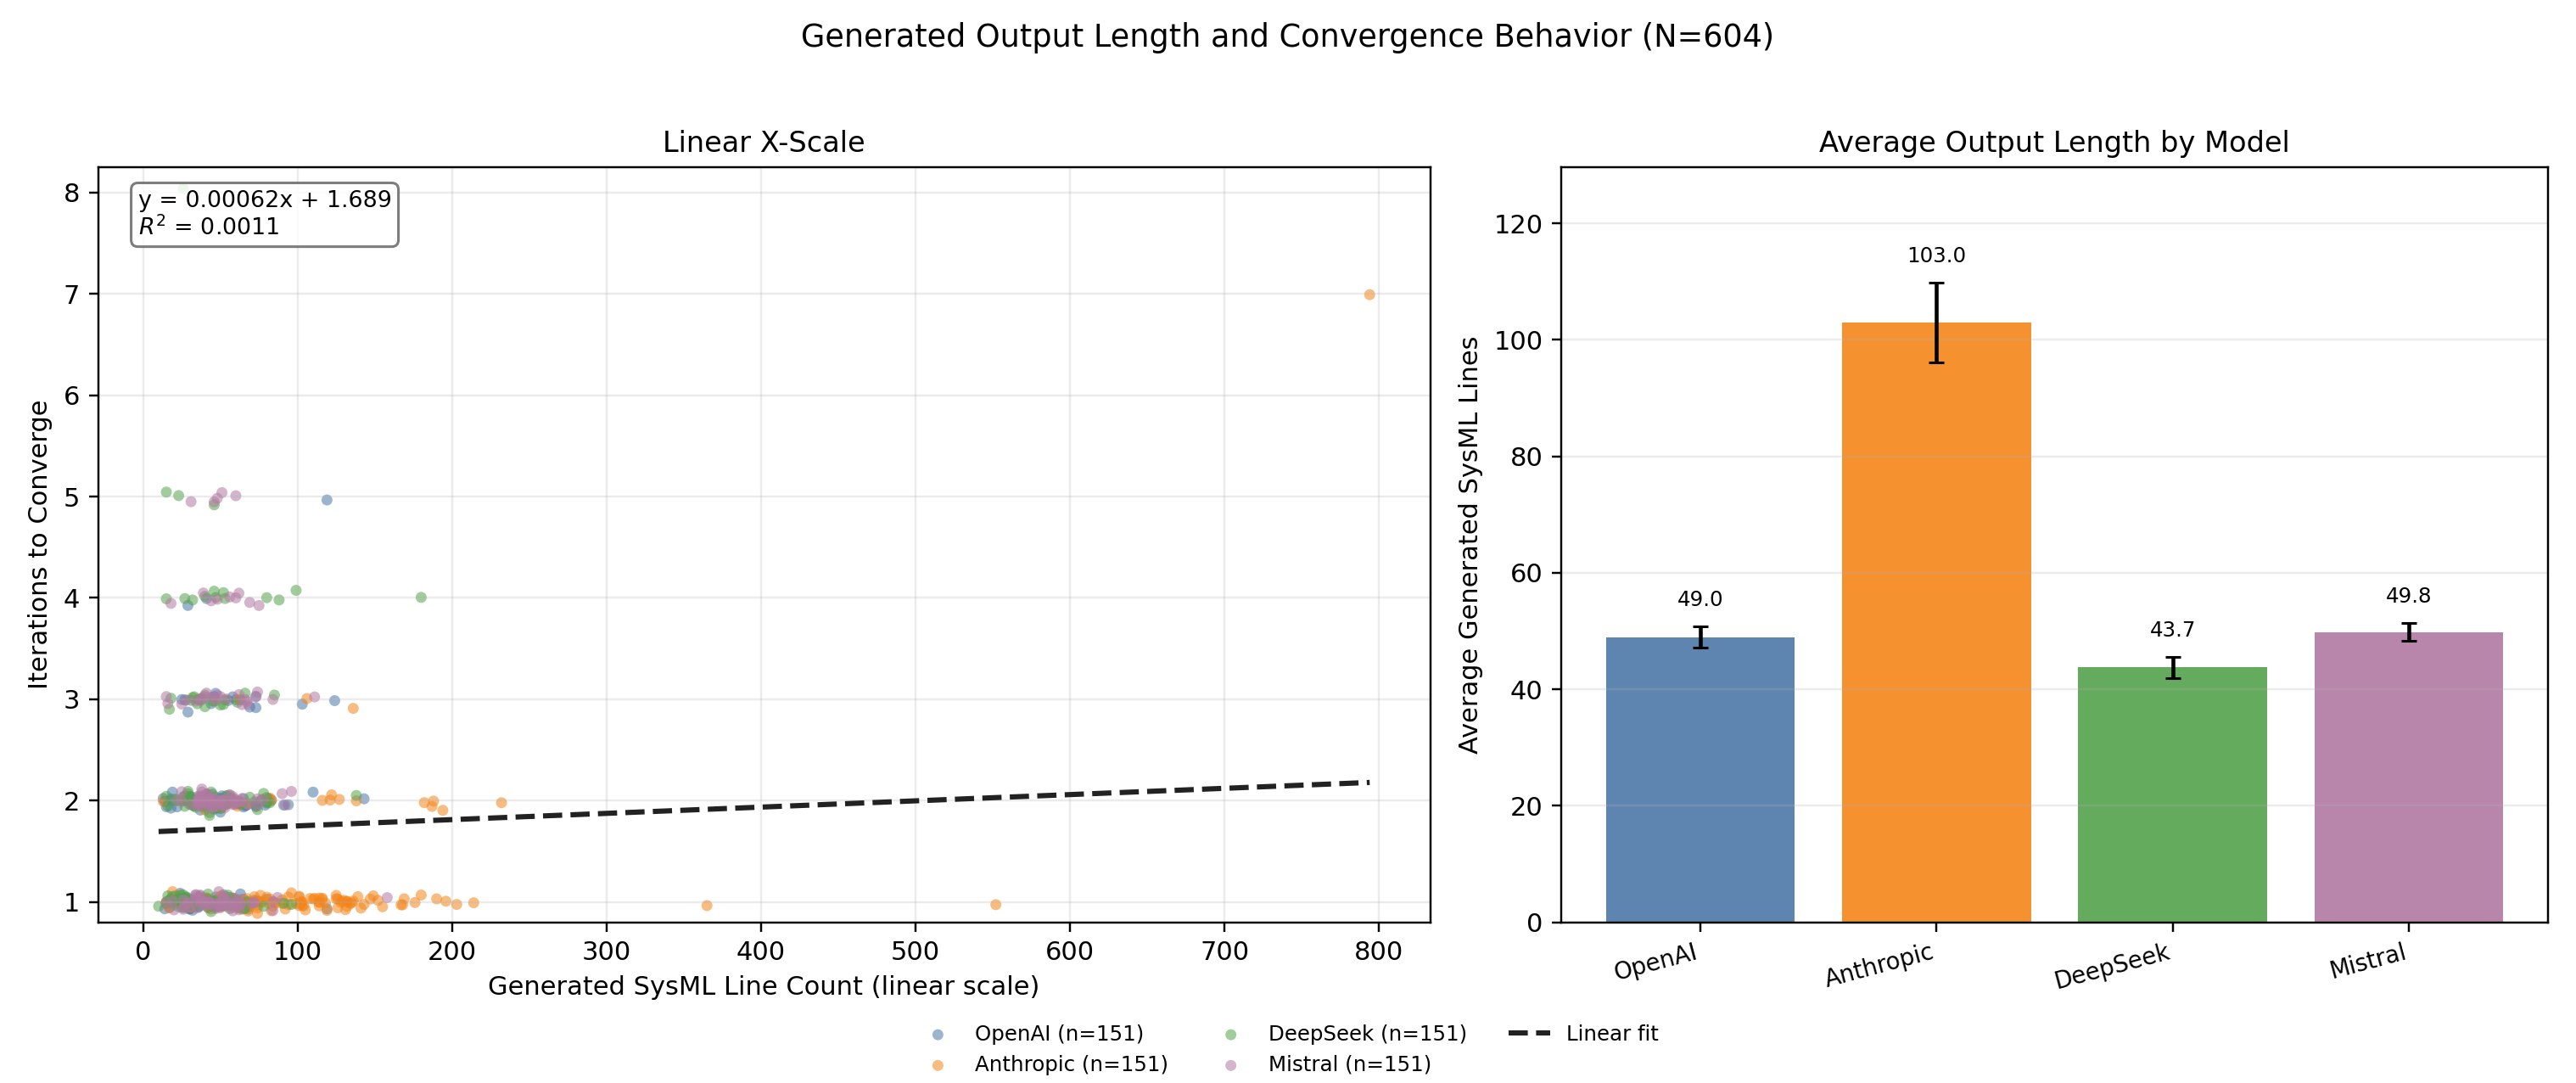
\includegraphics[width=\columnwidth,keepaspectratio]{appendix/appendix_additions/figures/fig14_generated_output_lines_vs_iterations_scatter_trend.png}
\caption{Generated SysML output length analysis. The left panel shows a scatter plot of generated SysML line count versus iterations-to-converge, with the pooled linear fit overlaid (\(R^2 = 0.0011\), slope \(= 0.00062\)). The right panel shows the average generated SysML line count for each model, with error bars indicating standard error.}
\label{fig:appendix_generated_lines}
\end{figure}

The pooled linear fit in Figure~\ref{fig:appendix_generated_lines} is essentially flat (\(R^2 = 0.0011\), slope \(= 0.00062\)), which indicates that generated SysML line count explains almost none of the variation in iterations-to-converge. In this analysis, generated output length is therefore not strongly correlated with repair effort.

The model-level averages in the right panel reinforce the same point. OpenAI, DeepSeek, and Mistral produce broadly similar output lengths on average (approximately 49, 44, and 50 lines, respectively), whereas Anthropic produces about 103 lines on average, or roughly twice as many. However, Anthropic also required the fewest iterations-to-success on average in the main results (1.23, versus 1.73 for OpenAI, 1.97 for DeepSeek, and 1.98 for Mistral), further indicating that line count alone is a poor standalone proxy for repair effort. Taken together, Figures~\ref{fig:appendix_difficulty} and~\ref{fig:appendix_generated_lines} suggest that repair effort is not well explained by size alone.

One possible explanation is that raw line count does not necessarily reflect the number of distinct syntactic structures that must be formed correctly. A model can generate many lines by expanding a relatively uniform pattern, whereas a shorter output may still involve a wider variety of declarations, references, and nested relationships that are more sensitive to validator failure. Simply producing more lines of the same structure therefore need not imply greater repair effort.

\section{Extended Analysis: Classifying Repair Attempts on Persistent Errors}
This appendix section looks at what the LLM does from one iteration to the next when a persistent error is still present. We treat an error as \emph{persistent} if an identical SysIDE diagnostic, meaning the same error family and the same \texttt{stderr} message, appears in two consecutive iterations of the same prompt-model run. To study the repair attempt itself, we compare the SysML artifact from iteration \(k\), which is the previous attempt fed back into the loop, with the revised SysML artifact produced by the LLM at iteration \(k+1\).

\subsection{Error Transition Outcome Explanations}
Using the SysIDE \texttt{stderr} outputs, we ask a simple question: when an identical error is still present at iteration \(k+1\), did the LLM appear to change the highlighted failing region, or did it leave that region unchanged? Across all back-to-back iteration pairs, this yields 1502 exact-error transitions. Each transition corresponds to one exact SysIDE diagnostic observed at iteration \(k\) and checked again at iteration \(k+1\). This is smaller than the total number of raw error instances because repeated copies of an identical SysIDE message within a single iteration are collapsed into one signature-level transition event. That choice is intentional: here we want to measure whether the model corrected an error pattern from one iteration to the next, not whether it repaired every repeated occurrence independently. We interpret many repeated identical grammar diagnostics as manifestations of the same underlying structural issue, so once the model applies the relevant pattern-level fix, repeated instances will often be corrected together rather than one by one.

Of these 1502 transitions, 1262 are resolved by the next iteration and are therefore not persistent. The remaining 240 persist through the next repair attempt. These 240 persistent transitions are the cases for which we want to understand whether the model tried to repair the highlighted region but failed, or whether it effectively carried the same failing code forward unchanged.

We then classify the 240 persistent cases into one of two categories:
\begin{itemize}
    \item \textbf{Unaddressed and not fixed}: an identical validator error remains at iteration \(k+1\), and the validator highlights an identical code snippet again.
    \item \textbf{Addressed but not fixed}: an identical validator error remains at iteration \(k+1\), but the validator now highlights a different code snippet instead, suggesting that the LLM changed the code to attempt to fix the error, but was unsuccessful.
\end{itemize}

To classify these persistent cases, we use the \texttt{stderr} outputs from SysIDE directly. For each persistent identical validator error, we compare the SysIDE \texttt{stderr} block at iteration \(k\) with the corresponding \texttt{stderr} block at iteration \(k+1\), and check whether SysIDE is still highlighting the identical code snippet or now highlights a different snippet instead.

For example, consider the following SysIDE \texttt{stderr} output. For readability, the long expected-token list is abbreviated here, but the full raw message is used in the analysis:
\begin{lstlisting}
iteration_01.sysml:36:19: error (parsing-error):
    Unexpected 'state', expected one of [...]
    36 |         attribute state : VehicleState;
       |                   ^^^^^
\end{lstlisting}
In this example, we classify the transition as ``unaddressed and not fixed'' only if iteration \(k+1\) still contains that identical \texttt{parsing-error} message and still highlights the identical code snippet, \texttt{attribute state : VehicleState;}. If iteration \(k+1\) still contains the identical \texttt{parsing-error} message but SysIDE now highlights a different code snippet instead, we classify the transition as ``addressed but not fixed.'' This is determined directly from validator stderr rather than by manually reading the full file.

A small amount of noise is possible for the ``addressed but not fixed'' category if multiple identical errors occur in different code regions within the same file. In that edge case, the LLM could fix one identical occurrence but fail to fix another identical occurrence on a different code segment, which would still appear here as ``addressed but not fixed.'' We expect this to be uncommon in practice, because many grammar repairs are pattern-level corrections that tend to fix repeated identical structures together.

\subsection{Persistent Error Analysis}
Figure~\ref{fig:appendix_persistent_transition_outcomes} restricts attention to the 240 persistent transitions and shows the split between the two persistent outcomes. Of these persistent cases, 155/240 (64.6\%) are ``unaddressed and not fixed,'' while 85/240 (35.4\%) are ``addressed but not fixed.''

\begin{figure}[H]
\centering
\definecolor{singleShotColor}{RGB}{196,106,28}
\definecolor{pipelineColor}{RGB}{44,138,100}
\begin{tikzpicture}
\begin{axis}[
    xbar,
    width=0.97\columnwidth,
    height=0.34\columnwidth,
    xmin=0,
    xmax=105,
    xlabel={Share of Persistent Transitions (\%)},
    symbolic y coords={Addressed,Unaddressed},
    ytick={Unaddressed,Addressed},
    yticklabels={{Unaddressed\\and not fixed},{Addressed\\but not fixed}},
    enlarge y limits={abs=4pt},
    axis lines*=left,
    xmajorgrids=true,
    grid style={dashed,gray!25},
    tick label style={font=\footnotesize},
    yticklabel style={align=right},
    label style={font=\footnotesize},
    nodes near coords={\pgfmathprintnumber[fixed,precision=2]{\pgfplotspointmeta}},
    every node near coord/.append style={font=\footnotesize, text=black, anchor=west, xshift=2pt},
]
\addplot+[fill=singleShotColor, draw=singleShotColor!70!black] coordinates {
    (64.58,Unaddressed)
};
\addplot+[fill=pipelineColor, draw=pipelineColor!70!black] coordinates {
    (35.42,Addressed)
};
\end{axis}
\end{tikzpicture}

\caption{Persistent exact-error outcomes among the 240 transitions for which an identical validator error remains present at iteration \(k+1\). Of these persistent cases, 155/240 (64.6\%) are unaddressed and not fixed, while 85/240 (35.4\%) are addressed but not fixed.}
\label{fig:appendix_persistent_transition_outcomes}
\end{figure}

The larger unaddressed-and-not-fixed share points to an inefficiency in the repair loop. In these cases, SysIDE is still highlighting the identical offending code region in the next iteration, suggesting that the LLM did not change that highlighted region after receiving the validator feedback. This motivates future work on stronger grounding of the prompt to the validator-highlighted snippet, or repair policies that explicitly require the highlighted region to be revised before resubmission.

The addressed-but-not-fixed share instead suggests LLM limitations. In these cases, the model appears to make a repair attempt, but the identical validator error still remains. This suggests a limitation in repair capability rather than simple loop inefficiency: the model changes the code, but does not produce a syntactically valid correction. Future work here should focus on constrained editing or fine-tuning with the large datasets of syntactically valid code that can now be produced. One caveat is that this analysis is based on SysIDE \texttt{stderr} and highlighted snippets, so rare repeated-identical-error cases can still add a small amount of noise.


\end{document}
